\chapter{Theorie}
\label{sec:Theorie}
\section{Definition der Reynoldszahl}
\label{sec:DefinitionDerReynoldszahl}
Die Reynoldszahl (Formelzeichen: $Re$) ist eine nach dem Physiker Osborne Reynolds benannte dimensionslose Kennzahl. Sie wird in der Strömungslehre verwendet und stellt das Verhältnis von Trägheits- zu Zähigkeitskräften dar (bzw. das Verhältnis von spezifischer Impulskonvektion zu Impulsdiffusion im System). Für eine ideale Flüssigkeit ohne Viskosität ist das Verhältnis unendlich.\par
Die Reynoldszahl definiert sich über die Gleichung
\begin{equation}
	Re= \frac{\rho_l u_b d_e}{\eta_l} \ \ \ \ \ \ \ \mbox{.}
\end{equation}
Überschreitet die Reynoldszahl einen (problemabhängigen) kritischen Wert ($Re_k$), wird eine bis dahin laminare Strömung anfällig gegen kleinste Störungen. Entsprechend ist für $Re~>~Re_k$ mit einem Umschlag, der so genannten Transition, von laminarer in turbulente Strömung zu rechnen.\par
In der Magnetohydrodynamik wird ebenfalls eine Reynoldszahl definiert: die magnetische Reynoldszahl.
\section{Anwendungen}
\label{sec:Anwendungen}
Die Abbildung \ref{fig:Reynoldsflugrpd} vergleicht Geschwindigkeiten und zugehörige Reynoldszahlen einiger Flugobjekte. Beispielsweise sind die Reynoldszahlen von Luftschiffen höher als die von Flugzeugen. Sie fahren zwar langsamer, sind aber deutlich größer.\par
Die Reynoldszahl ist eine wichtige Größe innerhalb der Ähnlichkeitstheorie. Will man zum Beispiel ein verkleinertes Modell eines Flugzeuges in einem Windkanal untersuchen, so muss der Wert der Reynoldszahl von Original und Modell gleich sein, um ein ähnliches Strömungsfeld zu erhalten. Entsprechend muss bei einem um einen Faktor $f$ verkleinerten Modell das Verhältnis $u/\widetilde{u} $ um den Faktor $f$ erhöht werden. Da die Maximalgeschwindigkeit begrenzt ist, senkt man in Kryo-Windkanälen zusätzlich die Viskosität der Luft durch Kühlung und erhöht dadurch gleichzeitig die Luftdichte. Auf diese Weise sind Reynoldszahlen bis zu $5\cdot10^7$ in Probenkammern von zwei Metern Durchmesser erreichbar. Dieses Vorgehen ist allerdings sehr teuer, da hier meist mit flüssigem Stickstoff der Kanal mitsamt Modell abgekühlt werden muss. Beim Abkühlen muss darauf geachtet werden, dass sich keine Vereisungen bilden. Eine weitere Erhöhung der Reynoldszahl kann auch durch die Erhöhung des statischen Druckes erreicht werden. 
\par
Staubkörner sind sehr klein. Wenn sie durch die Luft fallen, haben sie eine ähnlich niedrige Reynoldszahl wie eine Stahlkugel, die in ein Glas Honig fällt. Sie bewegt sich laminar (d. h. ohne Wirbelbildung) durch das Fluid. Ein Körper, der sich durch Wasser bewegt, hat bei gleicher Geschwindigkeit eine ca. 15fach höhere Reynoldszahl, als wenn er sich durch Luft bewegt. Zwar ist die dynamische Viskosität von Wasser ca. 50mal höher als die von Luft, jedoch ist auch die Dichte um das 800fache höher. 
Am Ende resultiert daraus eine höhere Reynoldszahl:
\begin{table}[htbp]
\caption{Kurze Tabellenüberschrift, generell mittig.}
	\label{tab:xyz}
	\centering
	\footnotesize
	\sffamily
		\begin{tabular}{|c||c|c|}
			\hline
			Substanz & Rel. dyn. Viskosität & Rel. Dichte \\ \hline\hline
			 Wasser  &          1           &      1      \\ \hline
			  Luft   &         0,02         &   0,0013    \\ \hline
			   x     &          y           &      z      \\ \hline
		\end{tabular}
\end{table}
\begin{table}[htbp]
\caption{Lange Tabellenüberschrift, welche länger als eine Zeile ist, wird linksbündig dargestellt. der Zeilenabstand reduziert sich zu eins.}
	\label{tab:xyz2}
	\centering
	\footnotesize
	\sffamily
		\begin{tabular}{|c||c|c|}
		\hline
		Substanz			& 	  Rel. dyn. Viskosität				&		Rel. Dichte				\\ \hline \hline
		Wasser				&			1														&		1									\\ \hline
		Luft					&			0,02												&		0,0013						\\ \hline
		x							&			y														&   z									\\ \hline
		\end{tabular}
\end{table}

Mikroorganismen schwimmen bei Reynoldszahlen $10^{-5}$ bis $10^{-2}$, so dass Inertialkräfte vernachlässigbar sind. Ein Beispiel: Hörten die Geißeln des Bakteriums E. coli auf zu schlagen, käme dieser Schwimmer bereits nach weniger als einem Atomdurchmesser zum Stehen.
\begin{figure}[htbp]
	\centering
		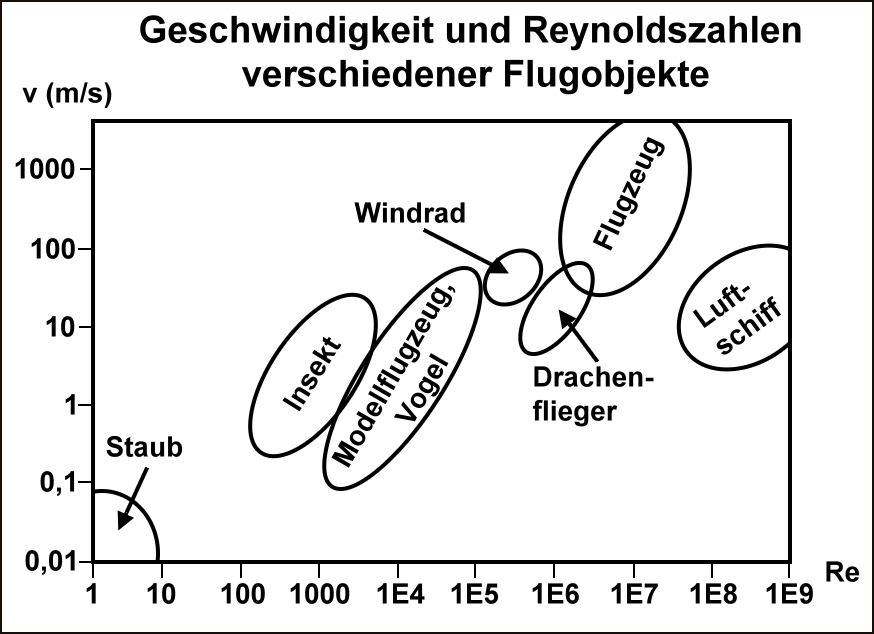
\includegraphics[width=0.80\textwidth]{Reynoldsflugrpd.png}
	\caption{Kurze Bildunterschrift}
	\label{fig:Reynoldsflugrpd}
\end{figure}
\begin{figure}[htbp]
	\centering
		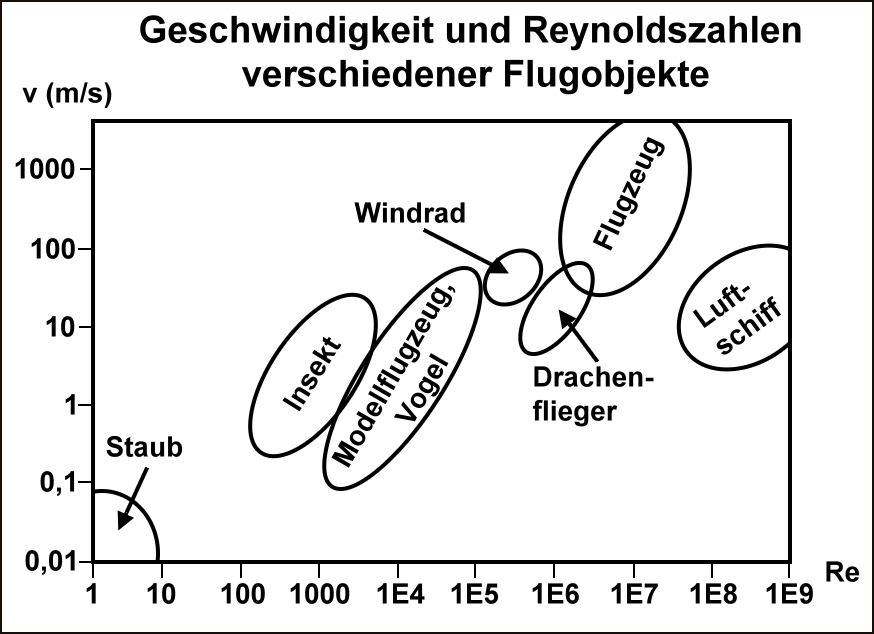
\includegraphics[width=0.80\textwidth]{Reynoldsflugrpd.png}
	\caption{Lange Bildunterschrift, welche die Länge einer Zeile überschreitet, bei mehrzeiligen Bildunterschriften wird der Zeilenabstand auf 1 reduziert.}
	\label{fig:Reynoldsflugrpd2}
\end{figure}
